% !TEX root = ../main.tex

\section{The Rust Programming Language} % (fold)
\label{sub:the_rust_programming_language}

{\rust}\footnote{\url{http://www.rust-lang.org/}} is a new open source systems programming language developed with backing from the Mozilla Foundation\footnote{\url{https://www.mozilla.org/en-US/foundation/}}.
It is a strongly and statically typed, multi-paradigm programming language that incorporates features from the functional, object-oriented, and imperative paradigms.
The language borrows many constructs and features from other programming languages, some of which are described in the following sections.
Over the course of {\rust}'s development, the language has set out to solve two major problems concerning both safety and concurrency, as well as taking full utilization of the underlying hardware.

\subsection{Language Features}
\label{ssub:rust:features}

This section starts by describing {\rust}'s standard library and its type-system, before moving on to presenting some of the language features that make {\rust} so different from {\C}.
Because {\rust} is a multi-paradigm language it offers a wider range of language constructs that are not present in the procedural paradigm usually found in embedded programming.

\subsubsection{The Rust Standard Library}
\label{sec:rsl}

The \gls{rsl} is included into all {\rust} programs and is an abstraction layer to write portable applications.
The library is implemented as a facade, meaning that \gls{rsl} provides a thin wrapper which reexports a stable interface for libraries like \lib{alloc} (for memory allocation), \lib{collections} (general purpose data structures) and {\core} (described in the next section).
Besides to providing the facade, \gls{rsl} defines platform abstractions like files, network protocols, and threading, all of which depends on an OS.
This basic fact renders the \gls{rsl} unusable in an embedded system as these dependencies will not be met.
It is possible to opt-out of using the library.

\subsubsection{The Rust Core Library}
\label{sec:rcl}

\gls{rcl} defines the platform independent part of the language.
This library is not intended to be directly interfaced with by the application programmer; instead a stable interface is reexported through \gls{rsl}.
In this way, \gls{rcl} is not interfaced with directly in normal {\rust} programs.
This gives the developer the ability to modify the library while the \gls{rsl} interface stays the same.

\autoref{tab:rust:datatypes} lists the primitive datatypes available in {\rust}.
\gls{rcl} defines many functions and abstractions that are used to manage and manipulate these datatypes.
The table shows that {\rust} is explicit about the size and signedness of integer data types, and that in addition to the Pointer/Array distinction made by {\C}, {\rust} also provides \concept{slices}, \concept{strings} and \concept{tuples}.

\begin{table}[H]
  \centering
  \begin{tabular}{r|l}
    \textbf{Type} & \textbf{Description} \\
    \hline
    \keyword{bool}  & Either \code{true} or \code{false} \\
    \keyword{char}  & A UTF-8 scalar value \\
    \keyword{f32}, \keyword{f64} & Floating point number of single and double precision \\
    \keyword{u8}, \keyword{u16}, \keyword{u32}, \keyword{u64} & Unsigned integers \\
    \keyword{i8}, \keyword{i16}, \keyword{i32}, \keyword{i64} & Signed integers \\
    \keyword{isize}, \keyword{usize}                        & `Pointer-sized' Integers \\
    Pointer        & Raw unsafe\footnote{Explained in \autoref{ssub:unsafe_code}} pointers (\code{*const T}, \code{*mut T}) \\
    Array          & Fixed-length array type, denoted with \code{[T]} \\
    \keyword{slice} & A view into a array, denoted with \code{\&[T]} \\
    \keyword{str}   & UTF-8 encoded byte array \\
    Tuple          & Finite ordered list of elements \\
    \hline
  \end{tabular}

  \caption{\rust's primitive datatypes}
  \label{tab:rust:datatypes}
\end{table}

% \paragraph{tuple}

% A tuple type is a fixed size datatype of variable types.
% The type can be used to return multiple return values from a function.
% In addition the type supports tags just like the variants of an enum.


\subsubsection{Variables and Bindings}

{\rust} features a handful of different data types, all of which can be assigned to a \emph{variable} using a \emph{binding}.
The most important types are described in the following sections, but we will first look at how variables work.
A value gets bound to a variable by utilizing the \keyword{let} keyword.
A variable in {\rust} has a name and a value, much like other programming languages, but there is a distinct difference between the \emph{mutability} of those variables.

With a mutable variable binding, it is possible to change the value of the variable.
However, if we try to alter the value of an immutable variable binding, {\rust} will give us a compile-time error.
The example code in \autoref{lst:rust_variable_bindings} shows how to declare both mutable and immutable variables and how to modify their values.
The example will not work because we attempt to change the value of an immutable variable.

\begin{listing}[H]
  \begin{minted}{rust}
// bind the value `5' to the immutable variable `a'
let a: i32 = 5;
// bind the value `10' to the mutable variable `b'
let mut b = 10;
b = a; // change the value of `b'
a = b; // <- compiler error: re-assignment of immutable variable `a'
  \end{minted}
  \caption{Variable bindings}
  \label{lst:rust_variable_bindings}
\end{listing}

An important part of variable bindings is {\rust}'s ability to automatically infer the data type of the variables.
We can see from the example that \code{a} is defined as a 32-bit integer with the value 5, and because the variable \code{b} later gets assigned to \code{a}'s value, {\rust} will automatically infer \code{b} to be of the same type.

\subsubsection{Enums}

An {\enum} in {\rust} (otherwise known as a sum type, or a tagged union, from type theory), is a data structure that is used to hold only one out of a small set of possible values.
\rust's {\enum} construct is a class of \emph{algebraic data types} that are common in functional programming languages, which means that its actual type is formed by combining other types together.
This makes the {\enum} a powerful feature of the language that can be used to deterministically limit the set of possible outcomes for a type.
\autoref{lst:rust:option} shows the definition of one of {\rust}'s most commonly used types which are used extensively throughout its standard library and other third party libraries and applications.

\begin{listing}[H]
  \begin{minted}{rust}
    pub enum Option<T> {
      Some(T),
      None,
    }
  \end{minted}
  \caption{Definition of Option}
  \label{lst:rust:option}
\end{listing}

Every \code{Option} variable is an {\enum} that can either have the algebraic value \code{Some} or the \emph{named value} \code{None}.
If the variable is \code{Some}, the definition also says that it needs to contain another type \code{T}.
This is also an example of generics in {\rust}, as \code{T} can be anything, e.g. an integer, a string, or a user defined type.
The \code{Option} type is analogous with a normal {\C} pointer value, which either has the value 0, or \code{null} (analogous to \code{None}), or a value that points to a structure at a place in memory (analogous to \code{Some}).
Even though the \code{Option} is analogous to a {\C} pointer, it is important to note their differences.
It acts more like a wrapper around a potential value, where its internal value is not \emph{directly} accessible, which encourages the programmer to handle the cases where it might be \code{None}.
The usage of {\enum} types described in this section become very expressive in combination with \keyword{match} expressions, as discussed in \autoref{sub:pattern_matching}.

\subsubsection{Structs}
\label{ssub:structs}

A \keyword{struct} in {\rust} is similar to that of {\C} and is a way of creating more advanced data types than primitives or enums.
With a \keyword{struct}, it is possible to combine multiple variables into a single type, each of them identified by its name.
An example of defining a \code{Book} is shown in \autoref{lst:book_struct}.
Anyone that is familiar with {\C} will see the similarity of the \keyword{struct} definition, but there is also a couple of extra things to notice from the example.
Everything in {\rust} is \emph{private} by default, but the \code{pub} keywords on type definitions and member fields make them \emph{publicly accessible}.
The \keyword{impl} keyword allows us to implement member functions for the \code{Book}, similar to class-declarations in {\Cpp} and other object-oriented languages.

\begin{listing}[H]
  \begin{minted}{rust}
    pub struct Book {
      pub name: String,
      pub pages: u32,
    }

    impl Book {
      pub fn info(&self) {
        println!("{} has {} pages.", self.name, self.pages);
      }
    }
  \end{minted}
  \caption{Struct definition and implementation}
  \label{lst:book_struct}
\end{listing}

\subsubsection{Pointers}

\rust's {\core} library exposes two pointer types that are considered \emph{unsafe} by the language, which \autoref{ssub:unsafe_code} explains.
Pointers in {\rust} are a fundamental part of the language, but they are not used much outside of low-level code and bindings.
Instead, the library offers higher-level structures as an abstraction between the \emph{raw} pointers and their data.

\subsubsection{Slices}

The \code{slice} type is simply a view into an array, and it is represented by a pointer and a length, as shown in \autoref{lst:rust:slice}.
The length is used to determine how many elements the slice represents.
Slice syntax is denoted by \code{\&[T]}, which reads like `a reference to a finite array with type \code{T}.'
They are a fundamental type that abstracts away the underlying block of data references by its internal pointer.

\begin{listing}[H]
  \begin{minted}{rust}
    pub struct Slice<T> {
      pub data: *const T,
      pub len: usize
    }
\end{minted}
\caption{Slice representation}
\label{lst:rust:slice}
\end{listing}

An example of a common slice type in {\rust} is the \keyword{str} type, which can either be a statically allocated string defined as a literal or a borrowed reference into another string.
The representation of the string type is closely related to slices, as a string slice denoted as \code{\&str} is equivalent to a UTF-8 encoded slice of bytes, denoted as \code{\&[u8]}.
It is important to note that an arbitrary slice of bytes is not necessarily a valid string.
% The \keyword{str} type differs from a \code{cstring} because it is guaranteed to be valid UTF-8, and it is \emph{not} null terminated.

\subsubsection{Boxed values}

\autoref{lst:rust:list} shows an example of how a linked list can be represented with an enum.
Each list item is either a value and a pointer to the next item, as in \code{Cons}, or a termination value, as in \code{Nil}.
One important thing to notice in this example is the usage of a \code{Box<...>} instead of the mentioned pointer.
As discussed earlier, {\rust} provides abstractions on top of its raw pointers, and the \code{Box} is an example of this in action.
A boxed value is simply a value that is stored on the heap, with its owning handle stored in a \code{Box} structure.
This structure implements the same operators that are otherwise associated with pointers, so they are semantically the same for this piece of code.

\begin{listing}[H]
  \begin{minted}{rust}
    enum List<T> {
      Cons(T, Box<List>),
      Nil,
    }
  \end{minted}
  \caption{Definition of Linked List}
  \label{lst:rust:list}
\end{listing}

\subsubsection{Pattern Matching and Destructuring}
\label{sub:pattern_matching}

Pattern matching is a powerful language construct of {\rust} that resembles the \code{switch} statement from {\C}.
It is possible to match against any value or variable in the language, and branch to different blocks of code based on the outcome of the \code{match}.
Another important feature of the \keyword{match} statement is that it needs to be \emph{exhaustive}, which means that all possible outcomes of a \keyword{match} need to be considered, otherwise {\rust} will issue an error during compilation.
This is contrary to {\C}, where only primitive values can be used in a \keyword{switch} statement, and there is no requirement to cover all switch cases, i.e. the \code{default} keyword is not required.

An example of pattern matching on the \code{Option} type is given in \autoref{lst:rust:match}.
We can see from the example that the match can be used to \emph{destructure} the matching value in order to get hold of its enclosing value.
We can also see that both \code{Some} and \code{None}, i.e. all possible outcomes of the \code{Option}, are being considered in the example.
% In Listing \ref{lst:rust:match} the Option \code{Some(42)} is checked against the patterns in the match expression.
% As the first pattern matches the value, the number \code{42} is bound to the variable number and the \code{println} function is executed.

\begin{listing}[H]
  \begin{minted}{rust}
    // Bind the value `Some(42)' to the variable `num'
    let num: Option<u32> = Some(42);

    match num {
      // Bind the Option's enclosing value to the variable
      // `number' and print its value
      Some(number) => println!("{}", number),
      // Otherwise do nothing
      None => (),
    }
  \end{minted}
  \caption{Matching an \code{Option}}
  \label{lst:rust:match}
\end{listing}

\subsubsection{Traits}

Traits in {\rust} are similar to Interfaces in Java - they are used to facilitate code reuse and polymorphism.
A \code{trait} can define a set of methods that other objects can implement, and in contrast to Java's Interfaces, a trait also supports default implementations for its methods that an object can inherit directly.
The definition of one of {\rust}'s more integral traits is the \code{Iterator} trait, which is shown in \autoref{lst:rust:iterator}.
An iterator can be used to manipulate stream- or list-like data structures, where the trait implements functions like e.g. \code{map}, \code{zip}, and \code{filter}, which are modifier functions that are commonly found in functional programming languages.

\begin{listing}[H]
  \begin{minted}{rust}
    pub trait Iterator {
      type Item;
      fn next(&mut self) -> Option<Self::Item>;
      fn size_hint(&self) -> (usize, Option<usize) { ... }
      // ...
    }
  \end{minted}
  \caption{Definition of the Iterator trait}
  \label{lst:rust:iterator}
\end{listing}

\subsubsection{Loops}
\label{sec:rust:loops}

{\rust} provides the two loop constructs known from {\C}, \code{for} and \code{while}, in addition to \code{loop} for infinite loops.
The \code{for} loop is not the conventional \code{for (initialize; condition; increment)} that is common in other languages, instead, it operates on iterators.
\rust's \code{for} statement is merely syntactic sugar for a \code{loop} with an internal \code{match} around the iterator's \code{next()} function.
\autoref{lst:rust:for} shows how a \code{for} loop is used to loop over a vector of numbers.
This code is de-sugared by {\rust} into the equivalent (simplified) code shown in \autoref{lst:rust:desugared-for}.

\begin{listing}[!h]
\begin{minipage}{0.45\textwidth}
  \begin{listing}[H]
    \begin{minted}{rust}
let values = vec![1, 2, 3];

for x in values {
  println!("{}", x);
}


    \end{minted}
    \caption{An iterator \code{for} loop}
    \label{lst:rust:for}
  \end{listing}
\end{minipage}
\begin{minipage}{0.45\textwidth}
  \begin{listing}[H]
    \begin{minted}{rust}
let mut it = values.into_iter();
loop {
  match it.next() {
    Some(x) => println!("{}", x),
    None => break,
  }
}
    \end{minted}
    \caption{{\rust}'s \code{for} loop de-sugared to a \code{loop}}
    \label{lst:rust:desugared-for}
  \end{listing}
\end{minipage}
\end{listing}

% \subsubsection{Case Study - Result}

% The Result type is an integral type in the {\rust} library and in {\rust} code in general.
% The type is the base type for error handling.

% \begin{listing}[H]
%   \begin{minted}{rust}
%     #[must_use]
%     pub enum Result<T, E> {
%       Ok(T),
%       Err(E),
%     }
% \end{minted}
% \caption{Definition of Result}
% \label{lst:rust:result}
% \end{listing}

\subsubsection{Closures}
\label{sec:back:rust:closures}

% Closures, a type of anonymous functions, exposes many expressive programming patterns which have emerged the last few years through the popularization of JavaScript \todo{Is this statement true? Maybe its gotten more recognized because of JS, but  closures have been around since at least the 70s...}, and several functional languages.
% The consquence is that both {\Cpp} and Java has added support for creating anonymous functions called lambda expressions.

A closure is an anonymous function that closes around the environment that it is defined within.
Any freestanding variables that are defined in this environment are accessible to the closure.
A closure can be used as an argument to another function, or be returned from a maker function.

\begin{listing}[H]
  \begin{minted}{rust}
fn main() {
  let (nums, limit) = (vec![1, 2, 3, 4], 3);
  let filtered: Vec<&u32> = nums.iter()
                                .filter(|&el| *el < limit)
                                .collect();
  println!("{:?}", filtered); // prints: `[1, 2]'
}
  \end{minted}
  \caption{Using a closure to filter the entries of a vector.}
  \label{lst:closure:filter}
\end{listing}

\autoref{lst:closure:filter} shows how a closure can be used to filter a list of numbers.
It also demonstrates one of the \code{Iterator} trait's many use cases.
The example initializes a vector with four numbers and makes an iterator by calling the \code{iter()} function.
Once the iterator is acquired, the \code{filter()} function is called with a closure as an argument.
The expression \code{|\&el| *el < limit} defines the closure, which takes an argument \code{el} and returns a \code{bool}.
The \code{limit} is a free variable that is found in the scope of the \texttt{main} function; this variable is part of the environment that is \emph{enclosed} by the closure.
When the \code{collect()} function is called, the closure is executed with every element in the vector, and they are collected into a new vector if the closure's condition is satisfied.


\subsection{Organization}
\label{ssub:rust:organization}

A {\rust} library or executable is organized into a \concept{crate}, and such a crate can consist of many \concept{modules}.
These modules are used to split up the library into separated pieces of code, which gives it a logical structure.
The crate is a shareable part of {\rust} code that can be included into other projects and libraries.
The modules are the hierarchical means of organizing a crate, and it ensures that the design is modular.
This gives the programmer the ability to import only the components of the library that is needed for a particular program.
\autoref{fig:rust:collections} shows a few of the modules contained within the {\rust} \lib{collections} crate.

\begin{figure}[H]
  \begin{center}
    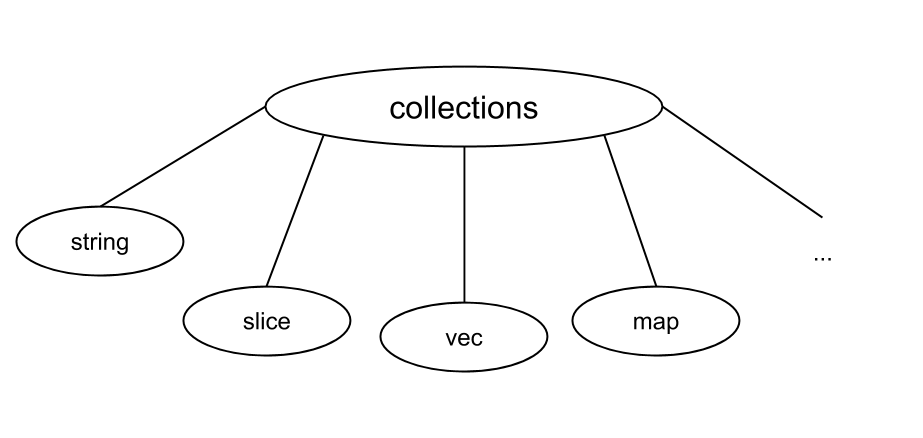
\includegraphics[scale=0.3]{figures/background/rust/libcollections.png}
  \end{center}
  \caption{Some of the modules in the \code{collections} crate}
  \label{fig:rust:collections}
\end{figure}

The {\rust} compiler comes bundled with a handful of standard libraries that are used as a basis for almost all third party libraries and executables.
By default, every {\rust} application is linked with the {\rust} {\std} library, which \concept{re-exports} functionality from the standard libraries, like e.g. the \lib{collections} crate.
%\todo{This figure looks broken...}
%\autoref{fig:rust:librust} shows some of the crates that make up the standard library, with their dependencies.
%Many of these libraries contains functionality that depends on an \gls{os} to be present, which is not necessarily a safe assumption to make for a bare-metal system.
%Because of this, the {\std} library can not be utilized in this project.
%Instead it have to be based on {\rust}'s {\core} library, which lays a foundation for all of the standard libraries, and does not depend on an \gls{os}.
%
%\begin{figure}[H]
%  \begin{center}
%    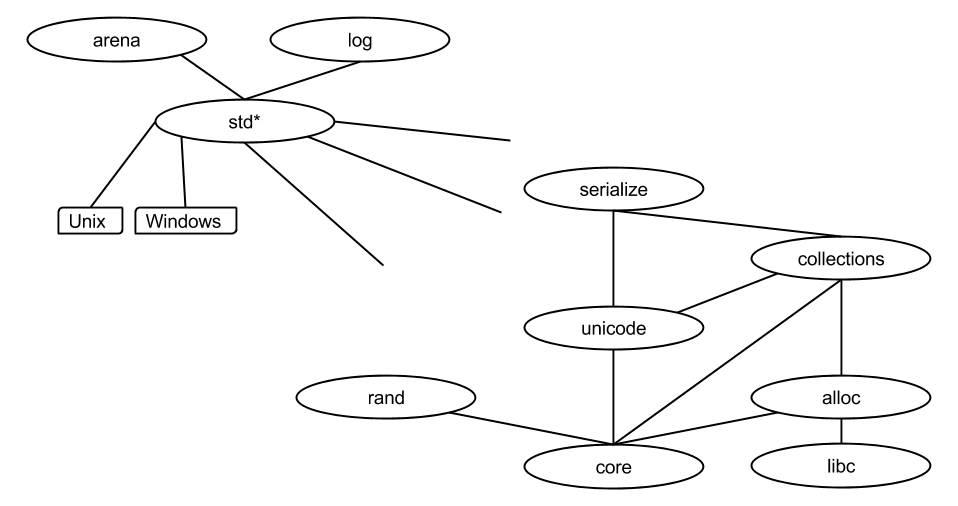
\includegraphics[scale=0.3]{figures/background/rust/rust-lib.png}
%  \end{center}
%  \caption{Some crates re-exported in the {\std} library}
%  \label{fig:rust:librust}
%\end{figure}

\subsection{Zero-cost Abstractions}
\label{chap:zero_cost_abstractions}

One of {\rust}'s goals is to achieve performance similar to {\C} and {\Cpp} while providing complete memory safety.
{\rust} aims to achieve this with \emph{zero-cost abstractions}, which means that the various high-level language constructs it implements does not come with an execution overhead.
This section gives a detailed example of one of {\rust}'s zero-cost abstractions.

Abstractions, in the form of references and pointers to objects or structures, and how they are
structured on the heap, is a common source of overhead in programming languages.
\autoref{fig:java_abstractions} shows how {\Java} lays out a vector of
strings in memory.
Fundamentally, a reference to the heap-allocated vector is placed on the stack, and the vector itself stores internal references to different strings that are placed elsewhere on the heap.
If we want to access the first character of a string stored in the vector, we would have to go through four levels of indirection - two objects need to be both dereferenced and indexed.
If the nesting of objects is deep, it can result in many heap-lookups in order to get the desired data.

\begin{figure}[tb]
  \begin{center}
    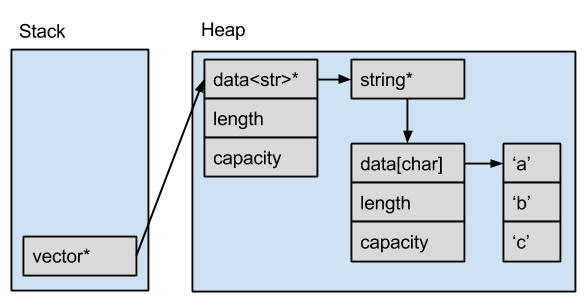
\includegraphics[width=0.8\textwidth]{figures/java_abstractions}
  \end{center}
  \caption{Abstractions of a Vector of Strings in Java.}
  \label{fig:java_abstractions}
\end{figure}

An important part of zero-cost abstractions is the ability to define new abstractions, like a vector, that optimizes away to the bare minimal.
{\rust} introduces the same zero-cost abstractions that are present in {\Cpp}, among other programming languages.
This is both important for performance, and for general purposes in order to have a deterministic and a common understanding of how the structures are laid out in the memory.
\autoref{fig:cpp_abstractions} shows how {\Cpp} places a vector of strings in memory.
The main difference is that the vector itself is placed on the stack, and the string data is placed directly inside the memory block owned by the vector.
The important part of this example is that we are keeping the same level of abstraction, but there are only two layers of indirection between the vector and the character data.

There is still one vital difference between the two examples.
We can safely have multiple references to our vector in {\Java} without worrying about what would happen if its memory would grow and reallocate.
However, we can end up with dangling pointers if we happen to have multiple references to our vector in {\Cpp}, and it grows and reallocates while we are holding such a reference.
\todo{Does this statement require further explanation? (i.e. explain why a reference to a stack-allocated vector in {\Cpp} can lead to a dangling pointer?}
In {\rust}'s case, all structures are allocated directly on the stack, if not explicitly told otherwise, which generally allows for faster access of data.
References to such stack-allocated variables can be passed around and accessed, just like in {\Cpp},
but {\rust} also introduces a set of rules that have to be followed to safely use these references.
These rules are based upon variable ownership and lifetimes, which are discussed in \autoref{sec:guaranteed_memory_safety}.
A {\rust} program will not successfully compile if the programmer fails to properly maintain these rules.

\begin{figure}[tb]
  \begin{center}
    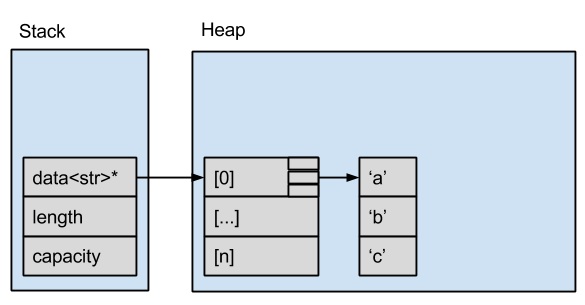
\includegraphics[width=0.8\textwidth]{figures/cpp_abstractions}
  \end{center}
  \caption{Abstractions of a Vector of Strings in {\rust} and {\Cpp}.}
  \label{fig:cpp_abstractions}
\end{figure}

\subsection{Guaranteed memory safety}
\label{sec:guaranteed_memory_safety}

One of {\rust}'s biggest features is its ability to maintain full memory safety without sacrificing performance.
The memory safety boils down to how {\rust} manages its variables and memory throughout the course of a program.
{\rust} introduces a few concepts that are all centered around the \concept{ownership} of these variables and their \concept{lifetimes}, and how references to these variables can be \concept{borrowed}.
These concepts are defined in {\rust}, but much of the inspiration behind those rules come from other type-safe languages, like {\lang{Haskell}} and {\lang{OCaml}}, and, in particular, {\lang{Cyclone}}'s \cite{Grossman2002,Swamy2006} region-based memory management.
{\rust}'s ownership system is part of all the zero-cost abstractions mentioned in \autoref{chap:zero_cost_abstractions}, since all borrow-checking and ownership- and lifetime-analysis are done statically during compilation.

\subsubsection{Ownership and Move Semantics}
\label{sec:back:rust:own}

To achieve full memory safety, we have to remove all forms for memory leaks and dangling pointers to invalid memory.
This implies one \concept{memory deallocation} for every respective \concept{memory allocation}.
Traditionally, when a programming language allocates memory for a variable, it will return a \emph{pointer} (or a \emph{handle}) and the number of bytes which is required to store the variable in memory.
This handle is essentially an address to a record in memory, and it can either be up to the language or the programmer to make sure that this memory is intact.
When the variable is no longer needed, the memory that is used by the handle can safely be deallocated.

Modern programming languages, like {\Java} and {\lang{Python}}, typically achieves this with a Garbage Collector that runs while the program is being executed with the sole purpose of keeping the memory intact.
A common implementation is a reference counted garbage collector \cite{Wilson1992} that keeps a count of the number of references to the variables and deallocates them when there are no valid references to them.
The downside of such an approach to memory safety is the continuous use of resources it requires to keep track of all the references.
The variables' reference counts must be altered every time they enter and leave a program scope.

Another common implementation is a stop-the-world garbage collector \cite{Wilson1992}.
It works differently by regularly halting the executing program before it recursively traces all references that are accessible from the \concept{root set} of variables.
The root set consists of global variables, local variables in the stack and any variable that may be available from the current state of the registers.
The memory that is accessible from these references are then marked as valid, and all the invalid memory will then become freed and accessible through new calls to the memory allocation function.
The downside of such an approach is the requirement of halting the entire program in order to release the invalid memory.
There are also many other techniques of garbage collection, which are often a variation of the ones already described.
However, they are all problematic in resource constraint environments such as on a small embedded device, or in real-time systems where the unpredictability of program execution introduced by a garbage collector is unacceptable.

Another approach to keeping track of the memory resources has been to give the programmer full control of every memory allocation and deallocation.
This is the most common approach for systems programming languages like {\C} and {\Cpp}, where performance and predictability are important.
However, it is easier to make the error of referencing invalid memory, or forgetting to free up memory that might lead the program to use all available resources over time.
Memory leaks like this will eventually lead a running program to crash due to the unavailability of extra resources.

It is important to always remember to deallocate all memory referenced by a handle before the handle leaves its scope in the program.
{\rust} operates differently from {\C} when it comes to freeing memory, any variables holding a reference to stack- or heap-allocated memory will automatically be freed when it leaves the scope it lives in.
This is done statically without any interference by the programmer.
When the compiler sees that the owning handle for the allocated memory leaves its scope, it knows that it is also lost to the program, so it will insert a call to free the memory right after it becomes unreachable.
This eliminates the need for the programmer to manually do the memory bookkeeping.
These two aspects of memory allocation and deallocation are combined into the concept of \concept{ownership} that {\rust} incorporates.
When a handle that \concept{owns} a reference to a data segment on the heap leaves its scope, {\rust} knows that it can safely free the memory that is referenced by it because it is the \concept{owning handle} to that memory.

\begin{listing}[tb]
\begin{minted}{c}
fn read_book(b: Book) {
  println!("You just read {} pages", b.pages);
}

fn main() {
  // `b' is the owning handle to a Book
  let b = Book { name: "Gecko's".to_string(), pages: 150 };
  // when this line is reached, `read_book' takes ownership of `b'
  read_book(b);
  // when `read_book' returns, the book is also deallocated
  // this makes it impossible to  read the book two times
  read_book(b); // <- compiler error: use of moved value: `b'
}
\end{minted}
\caption{Example of an owned handle}
\label{lst:owning_handle}
\end{listing}

An example of this ownership is shown in \autoref{lst:owning_handle}.
Only one owning handle can exist for any heap- or a stack-allocated variable at any time during program execution.
This means that if the handle gets passed as an argument to a function, this function will take \concept{ownership} of the variable by \concept{moving} it to the new scope defined by the function.
This move prevents any further use of the handle in its original scope and is necessary because {\rust} only allows one owned handle to any memory segment at any time.
If two or more handles to the memory had existed at the same time, it would have resulted in several calls to \func{free}, one for every time the handle left the different scopes.
The only way to continue using the handle in its original scope would have been to give the ownership back after using it.

\subsubsection{Borrowing}
\label{ssec:borrowing}

\concept{Borrowing} is introduced as an alternative to moving the variable ownership across multiple scopes.
{\rust} allows the programmer to \concept{lend} away access to handles by passing a reference to the variable around instead of the actual handle.
Multiple \emph{references} can exist to the same place in memory, as long as there is only one \concept{owner} of the actual handle.
A reference is denoted with an \code{\&} in front of the handle, which will tell {\rust} that we are working with a reference to the handle, or that we are borrowing the handle, to the end of the active scope.
Consider a modification of the previous example shown in \autoref{lst:borrowing_handle}.
Here, the \func{read\_book} function is modified to accept a reference to a book instead of overtaking its ownership, thus allowing us to lend out the book to be read as many times as we want.
Since the book's owning handle lives in the scope defined by the main function, the memory will be deallocated when the program exits.

\begin{listing}[tb]
\begin{minted}{c}
fn read_book(b: &Book) {
  println!("You just read {} pages", b.pages);
}

fn main() {
  // `b' is the owning handle to a Book
  let b = Book { name: "Gecko's".to_string(), pages: 150 };
  // only a reference to the book is given to `read_book'
  read_book(&b);
  // it is possible to read the book two times, because `b'
  // still lives in the scope defined by the `main' function
  read_book(&b);
 }
\end{minted}
\caption{Example of borrowing}
\label{lst:borrowing_handle}
\end{listing}

\subsubsection{Lifetimes}
\label{ssec:lifetimes}

{\rust} needs a way to ensure that the memory used by all borrowed references to a handle is intact, i.e. that the references do not point to any deallocated memory.
{\rust} achieves this with a concept called \concept{lifetimes}, in which the compiler, with the help of \emph{lifetime specifiers}, can statically resolve any dangling pointers or \concept{use-after-free} issues introduced by the programmer.
Consider the example shown in \autoref{lst:invalid_ref_c}, which shows a function in {\C} that returns a reference into a variable allocated in its own stackframe.
When the function returns, the variable will be de-allocated, and the returned reference will point to invalid memory.
The {\C} compiler is likely to issue a warning of such a serious mistake, but it will still compile the program.
A similar implementation of \code{name\_as\_ref} in {\rust} is shown in \autoref{lst:invalid_ref_rust}, but this will issue a compilation error because we try to return a reference without a lifetime specifier.

\begin{listing}[tb]
\begin{minted}{c}
char *name_as_ref() {
    Book b = { .name = "Gecko's", .pages = 150 };
    return &b.name;
}

int main() {
  char *name = name_as_ref();
}
\end{minted}
\caption{Returning an invalid reference in {\C}}
\label{lst:invalid_ref_c}
\end{listing}

\begin{listing}[tb]
\begin{minted}{rust}
fn name_as_ref() -> &str { // <- compiler error: missing lifetime specifier
    let b = Book { name: "Gecko's".to_string(), pages: 150 };
    &b.name
}

fn main() {
  let name = name_as_ref();
}
\end{minted}
\caption{Attempting to return an invalid reference in {\rust}}
\label{lst:invalid_ref_rust}
\end{listing}

An example of the same function, but with applied lifetime specifiers, is shown in \autoref{lst:valid_ref_rust}.
We can see from this example that {\rust} requires us to annotate all references that are associated with the function's arguments and return values with a name.
In this case, we have chosen the name \code{'a} for the lifetime specifier.
The explicit name of the lifetime does not matter, what matters is that {\rust} forces us to allocate the book elsewhere so that it is alive in the stackframe that encloses the function call to \code{name\_as\_ref}.
Note that this example just demonstrates what lifetime specifiers look like in {\rust} and shows one way the language can catch use-after free errors.

Another thing to notice is that the usage of lifetime specifiers in this example is somewhat verbose.
{\rust} will often let us elide the lifetimes associated with the variables completely, so we can usually get by without annotating the lifetimes like this.
The reader is encouraged to see The Rust Programming Language Book \cite{web:rust_book} for an in-depth explanation of {\rust}'s ownership- and lifetime-system.

\begin{listing}[tb]
\begin{minted}{rust}
fn name_as_ref<'a>(b: &'a Book) -> &'a str {
    &b.name
}

fn main() {
  let b = Book { name: "Gecko's".to_string(), pages: 150 };
  let n = name_as_ref(&b); // no use-after-free error
}
\end{minted}
\caption{Retuning a reference with correct use of lifetime elisions}
\label{lst:valid_ref_rust}
\end{listing}

% \subsection{Concurrency Model} % (fold)
% \label{ssub:concurrency_model}

% Solving both memory safety and concurrency might sound like two entirely different problems, but the ownership system described in \autoref{sec:guaranteed_memory_safety} actually turned out to go a long way of being the solution of them both \cite{web:fearless_concurrency_with_rust}.
% While we do not utilize or focus on the concurrency of {\rust} in this project, it is still a very important feature for the language, so it will be shortly introduced in this section.

% As already mentioned, {\rust}'s ownership system helps us to reason about the liveliness of variables, and it helps us to catch errors like use-after-free, and data races by not allowing us to have multiple references to the same mutable data.
% This makes it possible to describe and utilize many powerful idioms and paradigms, and concurrency models that are based on these core features of the language.
% Thus, {\rust}'s way of providing concurrency is made possible because the ownership system guarantees that it will be safe.
% Indeed, the core concurrency functionality in {\rust} is merely an abstraction that is defined in the standard library, is is not a feature in the language itself.
% This is an important distinction, because it allows for any number 3rd party concurrency libraries to evolve based on the same core principle of ownership, without being dependent on the concurrency idioms provided in the standard library.

\subsection{Unsafe Code} % (fold)
\label{ssub:unsafe_code}

{\rust}'s strong type system and static guarantees about memory safety goes a long way in verifying the safety of programs, but for certain programs, the restrictions set by the compiler might be too conservative.
Many programs that exist are indeed safe, but still not possible for the compiler to verify.
Examples of code that the compiler cannot verify is code that dereference \concept{raw pointers}, or code that utilize {\rust}'s \gls{ffi} or directly call on any of the compiler intrinsics functions.
Raw pointers in {\rust} are similar to normal pointers in {\C}, which means that they are not constrained by {\rust}'s ownership rules, and thus allows for aliasing to mutable data - they are not even guaranteed to have non-null values.
The compiler can not protect against use-after-free errors or dangling pointers when raw pointers are involved.

The ability to define new abstractions with efficient implementations is an important goal of {\rust}.
Sometimes, this means that the underlying code needs direct memory access and the ability to dereference raw pointers or call into external libraries.
For these tasks, {\rust} provides the keyword {\unsafe}.
It is important to note that this {\unsafe} keyword is introduced to \emph{keep} {\rust}'s semantics about memory safety.
When the compiler can no longer guarantee safety, it is up to the programmer to tell the compiler that the code inside the {\unsafe} block is indeed safe.

\begin{table}[ht]
\begin{center}
\begin{tabular}{p{4cm}|p{7cm}}
  \raggedleft{\textbf{Unsafe Operation}} &
  \textbf{Why it is considered unsafe} \\
  \hline
  \raggedleft{Access and update static mutable variables} &
  Writing and reading to and from global state can lead to race conditions because every thread and scope in the program has direct access to these global variables at the same time. \\

  \raggedleft{Dereference raw pointers} &
  There are no variable bindings between a raw pointer and the data it points to; thus the normal ownership rules provided by the borrow-checker does not apply to them. This means that {\rust} cannot resolve issues with race conditions or dangling pointers. \\

  \raggedleft{Call unsafe functions, e.g. \\ \gls{ffi} or compiler intrinsics} &
  {\rust} can make no guarantees about the safety of {\unsafe} functions. If a \gls{ffi} function is called, we are leaving {\rust}'s scope and entering another language domain, and it is not possible for {\rust} to verify the safety of such code. \\

\hline
\end{tabular}
\caption{Unsafe operations exposed through an {\unsafe} block}
\label{tab:reasons_for_unsafe}
\end{center}
\end{table}

\autoref{tab:reasons_for_unsafe} summarizes the three things that are possible to do in an {\unsafe} block, and some examples of why the operations are considered unsafe.
Compiler Intrinsics are functions that are provided by the compiler itself, not {\rust} and are functions that are closely related with raw pointers.
These are all considered unsafe, as they provide core functionality to e.g. access and modify volatile data, transform the data of one type into another, or perform atomic operations.

It is important to note that {\rust}'s borrow-checker is still active \emph{across} the unsafe code and that normal ownership rules still apply even though the code is unsafe.
The borrow-checker can never be disabled, but for certain operations it will simply not work.
\autoref{lst:unsafe_reference} demonstrates this with the same example that was used in \autoref{ssec:lifetimes}.
We can see from this example that it is not allowed to return a reference to something that is allocated \emph{within} an unsafe block, as this can result in use-after-free issues.
This also tells us that using an unsafe block is not the same as disabling the compiler, it is merely a mechanism for the programmer to handle the safety of a program in the cases where the compiler is unable to.

\begin{listing}[H]
\begin{minted}{rust}
fn main() {
  let name = unsafe {
    let b = Book { name: "Gecko's".to_string(), pages: 150 };
    &b.name // <- compiler error: `b.name' does not live long enough
  };
}
\end{minted}
\caption{Attempting to return an invalid reference from an \code{unsafe} block}
\label{lst:unsafe_reference}
\end{listing}
